\chapter{Material}
\section{Das Rennrad}

\section{Regelmässige Wartung des Rades}
Pannensicherheit Rennvelo. Vorsorge.
\begin{figure}[htpb]
        \centering
        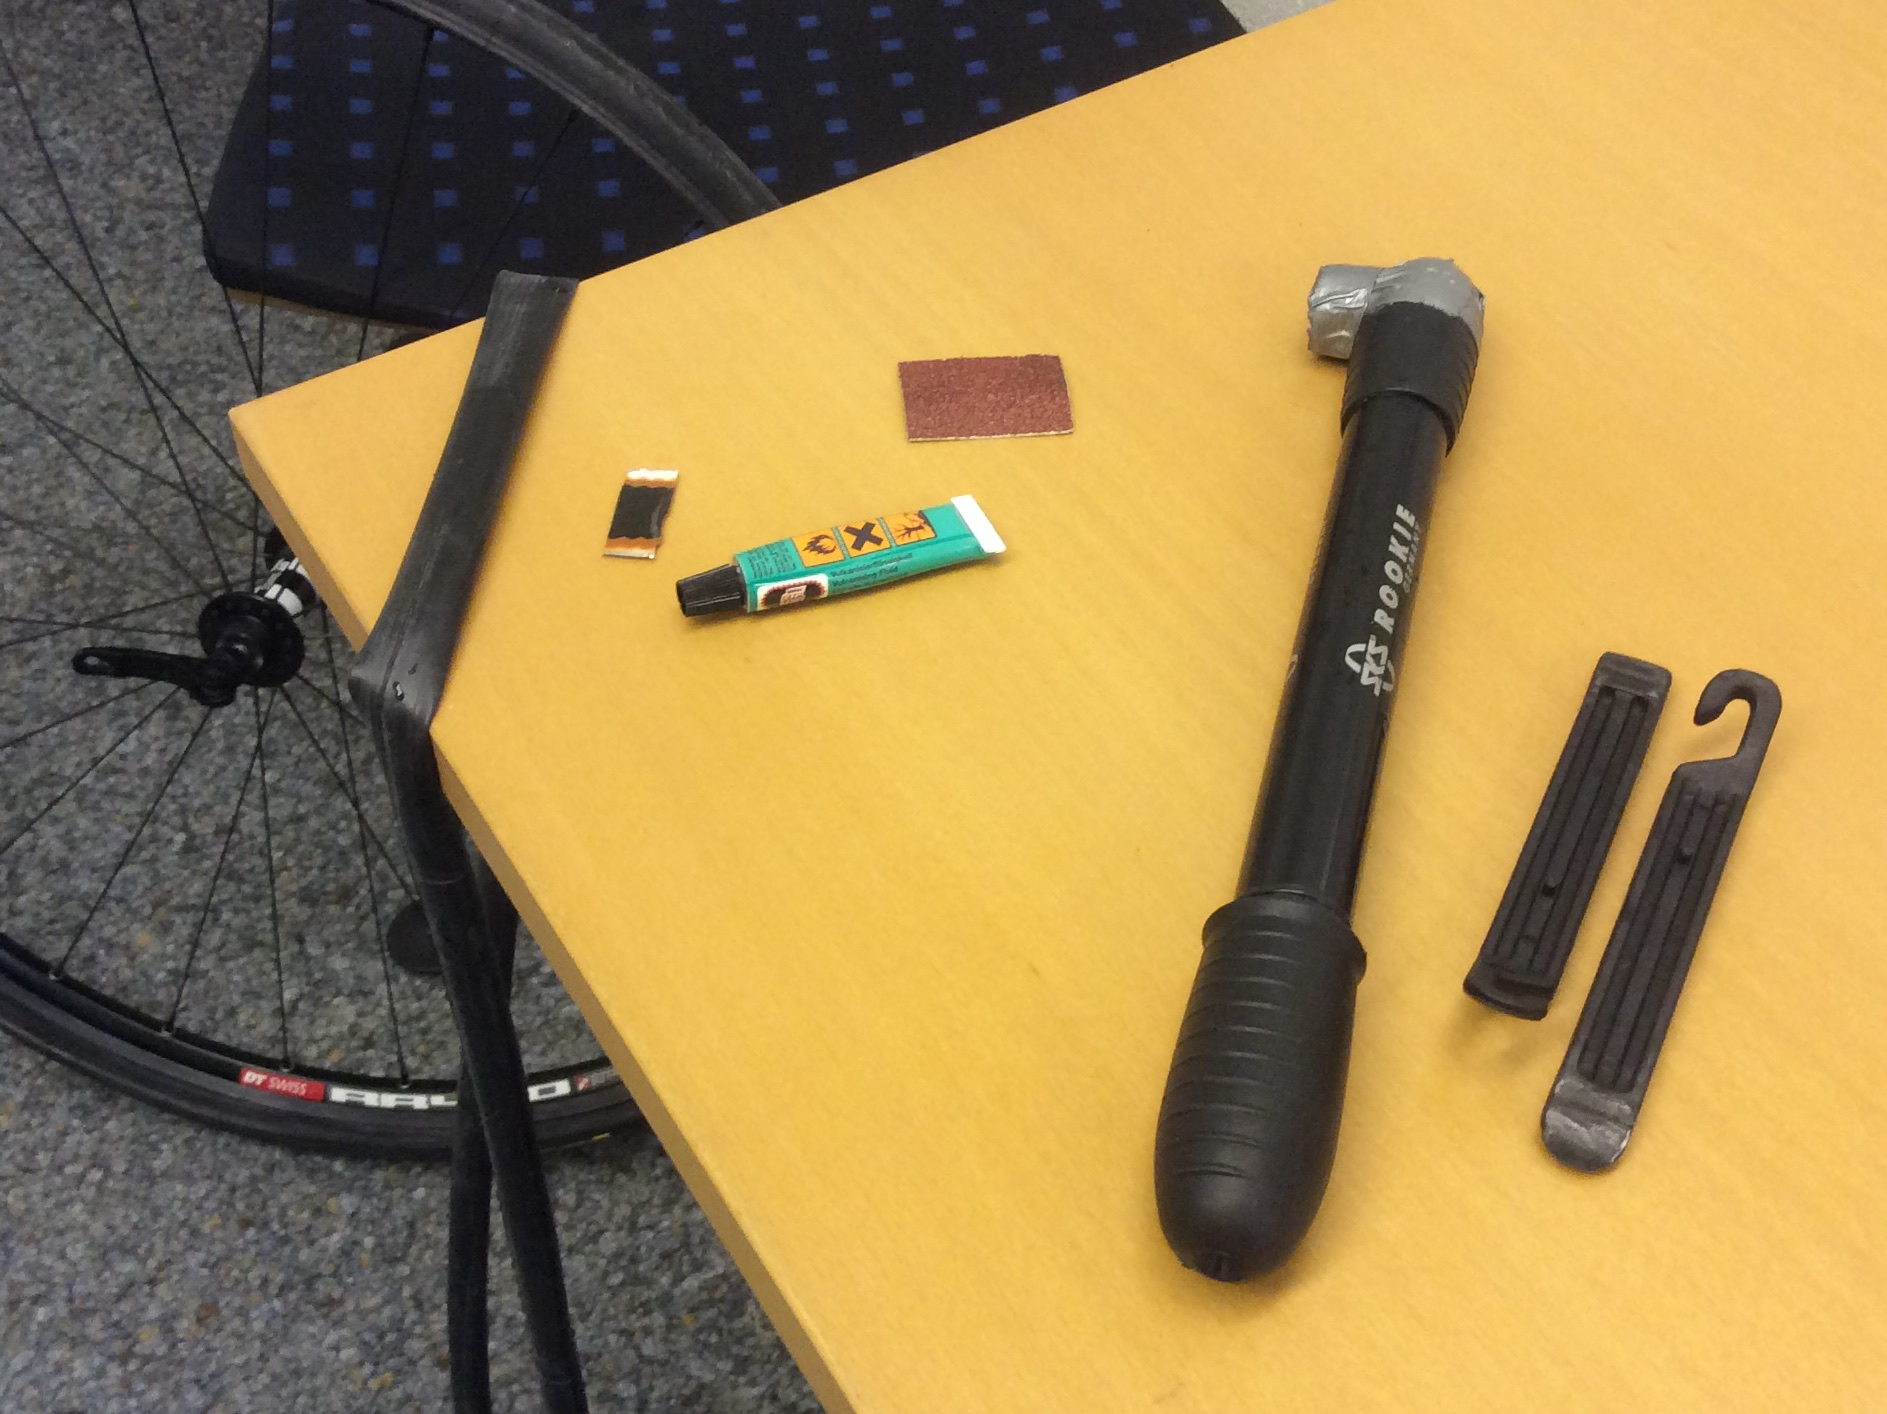
\includegraphics[width=\textwidth]{figures/reparatur-arbeitsplatz.jpg}
        \caption{Reparatur am Arbeitsplatz}
        \label{fig:reparatur-arbeitsplatz}
\end{figure}


\section{Wieso ein Rennrad zum Pendeln}

Es gibt durchaus Gründe, wieso man eher ein Trekking- oder Fitness-Bike als ideales Pendler-Rad sehen kann \cite{Lindthaler2015perfektesfahrradpendler}.



Möglichkeit der Reparatur unterwegs oder am Zielort (Arbeitsplatz, zu Hause). Möglichkeit einer Alternative (ÖV, Taxi).
Reparatur am Arbeitsort
Gelegentlich passiert einem etwas auf dem Weg zur Arbeit. Wenn man das Rennvelo dann reparieren kann, erspart man sich viel umtriebe (Transport des nicht mehr fahrtauglcihen Rades nach Hause, dortige Reparatur). Kleine Reparaturen wie platter Reifen usw. macht man am besten in einer Arbeitsplause oder über Mittag.
Regeneration, Wiederherstellen des Betriebszustand

Das Rennrad muss regelmässig gewartet werden.

Kleine Reperaturen deshalb gleich am Abend machen, am Wochenenden oder freien Tagen einen umfassenden Check (Bremsen, Kette) und Unterhaltsarbeiten.
Je länger man mit Wartungsarbeiten zuwartet, desto umfagreicher werden erfahrungsgemäss die Reparaturen.
Auch eine wichtige Erfahrung: wenn einem beim Fahren etwas auffällt (Geräusch, komisches Gefühl), dann sollte man unbedingt dem nachgehen.
Ignorieren oder Verdrängen (<<Da wird schon nichts sein>>) bringt \emph{todsicher} Probleme.
Irgendwann ist dann die lockere Schraube ganz weg und eine Reparatur, die bei besserer Aufmerksamkeit ein paar Sekunden gedauert hätte,
wird ein Steckenbleiben am blödsten Ort und eine umfangreiche und teure Reparatur.


\section{Bekleidung}

Der Fokus ist hier eher bei Outdoor-Bekleidung als bei \emph{richtiger}, d.h. wettkampforienierter Rennradbekleidung.

Schuhe mit weicher Sole

Übershuhe als Regenschutz.

\section{Restliches Material}



